\chapter{Results}

\section{Usage Statistics}

A total of 28 students registered to use the software and 7,879 total reviews were recorded
by 3 November 2012.

Students showed interest in the software during the introduction in class, however many
students registered and used the software only once. Figure \ref{fig_visits} shows the initial
interest in the software as a spike in the number of visits toward the beginning of semester.
This graph tracks all visits including users that have not yet registered.

\begin{figure}[h!]
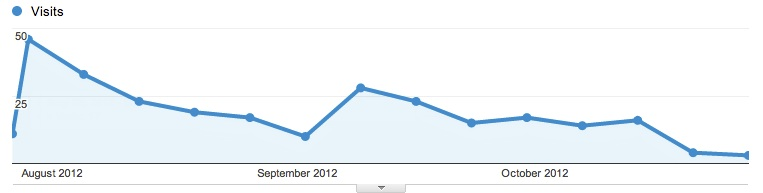
\includegraphics[width=12cm]{img/visits.jpg}
\caption{Google Analytics data on total number of visits to the application}
\label{fig_visits}
\end{figure}

Figure \ref{fig_usage_devices} shows most students accessed the software from a
desktop computer, while a handful accessed the
software exclusively from a mobile device. A single user accessed the software from both
a desktop and mobile device.

\begin{figure}[h!]
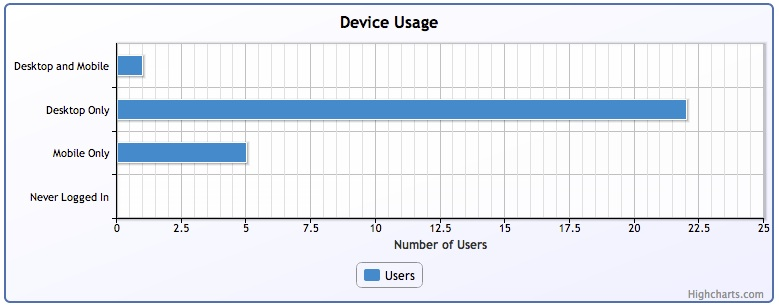
\includegraphics[width=12cm]{img/usage_devices.jpg}
\caption{The number of users according to the device used to access the software.}
\label{fig_usage_devices}
\end{figure}

The number of reviews completed per user is one of the more important statistics as
it shows the diversity of `useful' review data. Too many first reviews are useless as
they contain no useful data on which to later predict an answer.
Figure \ref{fig_usage_reviewcount} shows that eight users only completed new
reviews (the 1-20 range) after registering.

For the purposes of the following graphs, users were classified as `active' or `inactive'
based on the number of total reviews completed, with active users considered as those
who completed more than 200 reviews.

\begin{figure}[h!]
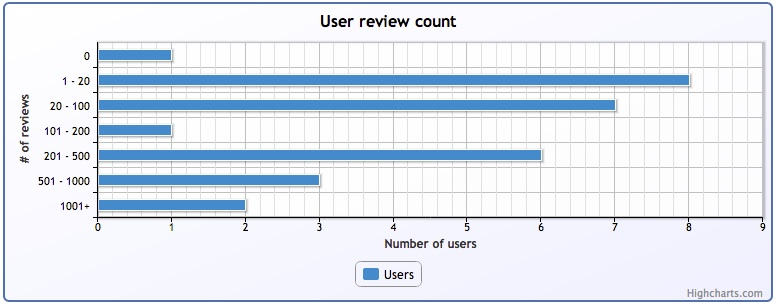
\includegraphics[width=12cm]{img/usage_reviewcount.jpg}
\caption{Number of users per total reviews. Users who had completed 
at least 200 reviews were considered `active users'.}
\label{fig_usage_reviewcount}
\end{figure}

Figure \ref{fig_usage_semester} shows the average number of reviews per user across the
semester. Users were divided up into `active' and `inactive' groups to avoid inactive
users skewing the data, though an average across all users is also shown with the blue line.

\begin{figure}[h!]
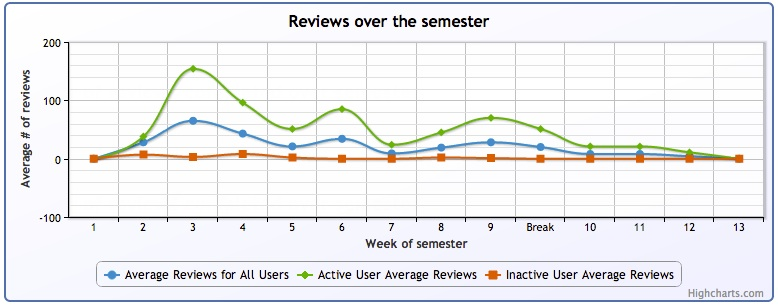
\includegraphics[width=12cm]{img/usage_semester.jpg}
\caption{Usage of the system over the semester.}
\label{fig_usage_semester}
\end{figure}

Users tended to complete most reviews on their first few days after registering,
with the most on the very first day. Figure \ref{fig_usage_sinceregistering} groups
reviews by the number of days since registering, showing a very fast dropoff in
number of reviews in the first couple of weeks after registering.

\begin{figure}[h!]
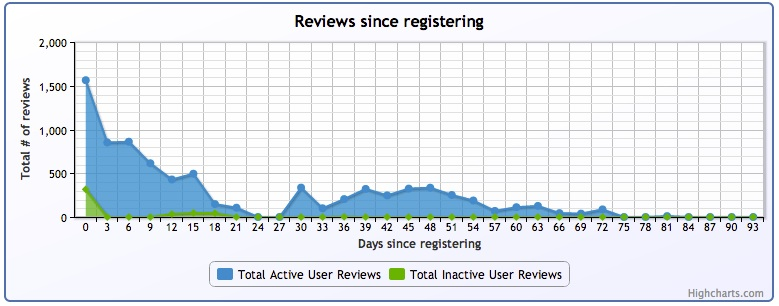
\includegraphics[width=12cm]{img/usage_sinceregistering.jpg}
\caption{Usage of the system shown as the number of days since registering.}
\label{fig_usage_sinceregistering}
\end{figure}

Figure \ref{fig_usage_sinceregistering} shows the total number of reviews per user
after registering. Only a few users registered in the second week of semester,
 with many more registering in the following weeks. However many users only
 completed reviews in the first few days after registration and stopped usage after
 that.
 
Only a few users used the software regularly; table \ref{tbl_topusers} shows the
statistics for the top five users by number of reviews.

\begin{table}[h!]
\caption{Top users and study statistics}
\label{tbl_topusers}
\begin{tabular}{|c|c|c|c|}
\hline
User ID & Number of logins & Vocabulary studied & Total reviews \\
\hline
20 & 59 & 100\% & 1910 \\
10 & 13 & 75\% & 1337 \\
21 & 13 & 45\% & 831 \\
19 & 9 & 50\% & 781 \\
26 & 9 & 58\% & 718 \\
\hline
\end{tabular}
\end{table}

\section{Forgetting Curves}
\subsection*{Generated from Recorded Reviews}

Figure \ref{fig_expforgetcurve} shows the review data grouped
as data points by the review number and days since previous review (actual interval).
The threshold $n$
is the number of reviews required for a data point to be displayed.

The progression from $n \geq 5$ to $n \geq 100$ shows a significant reduction of noise
in the data points, where $n$ is the number of reviews required to generate a single data
point. Ideally this threshold would be much higher, however with the limited data set
available increasing the threshold any more would reduce the number of data points
visible.

\begin{figure}[h!]
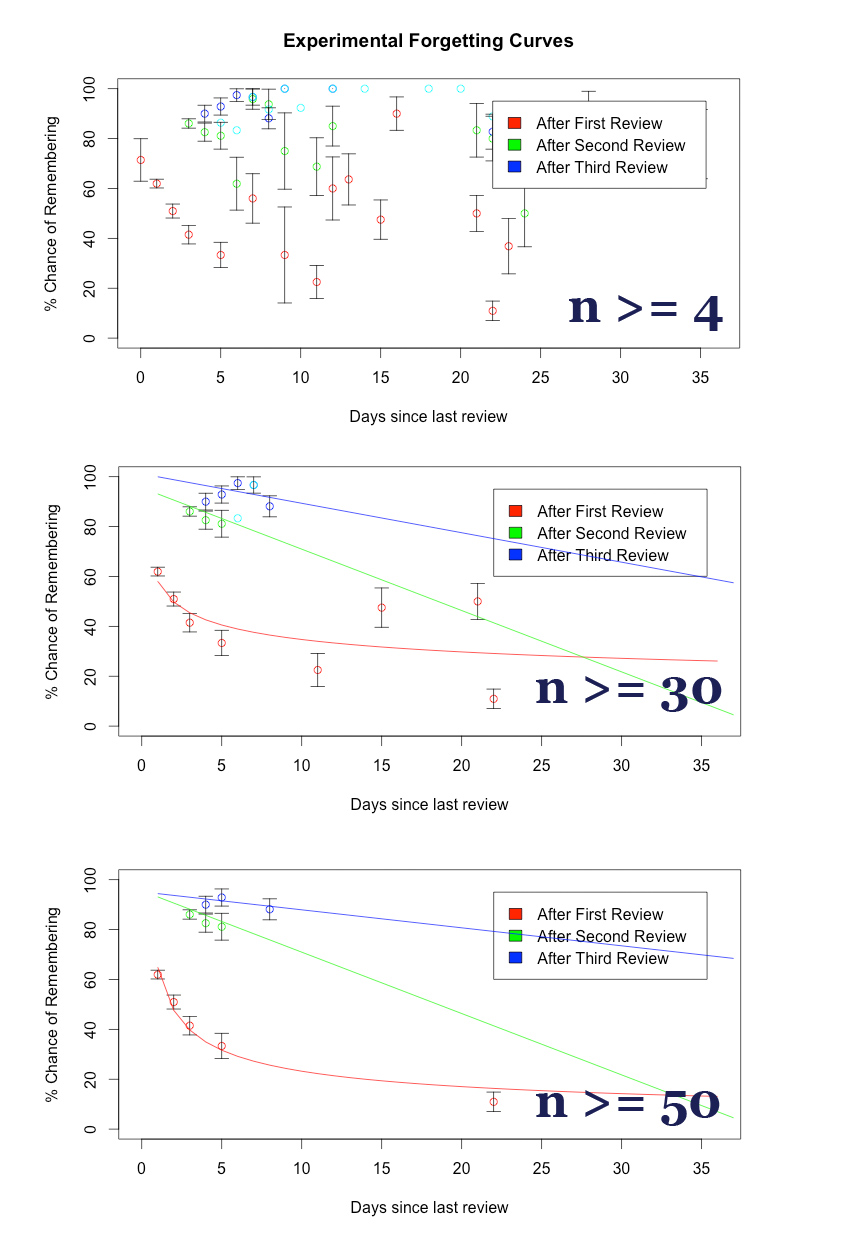
\includegraphics[width=14cm]{img/forgettingcurves.jpg}
\caption{Forgetting curves produced from recorded review data with threshold $n \geq 5$}
\label{fig_expforgetcurve}
\end{figure}

A much larger number of reviews were available for the first review, so the standard error
is reduced. The standard error as shown on the $n \geq 30$
graph in figure \ref{fig_expforgetcurve} for the first
data point is 1.7\% with the chance of remembering calculated from $n = 774$ review samples.
In contrast, the data point at fifteen days for the first review was calculated from only 
$n = 40$ available review samples, and has a standard error of 7.9\%.
\newpage
\subsection*{Generated from Machine Learning Algorithms}
Todo ????

\section{Prediction of Recall}

The machine learning algorithms tested averaged just under 70\% accuracy, with
the best performance on the validation set by the radial kernel based support vector
machine at 70.1\%.

Table \ref{tbl_algo_comparison} lists the algorithms tested and the accuracy of
classification on both the training and validation sets.

\begin{table}[h!]
\caption{Comparison of the performance of various machine learning algorithms on the output `Correct'. Accuracies are averaged over 15 runs.}
\label{tbl_algo_comparison}
\begin{tabular}{|p{5cm}|c|c|}
\hline
Algorithm & Training set accuracy & Validation set accuracy \\
\hline
Linear SVM & 69.41\% & 68.92\% \\
Radial SVM & 71.55\% & 70.14\% \\
Neural Network (Linear, 9 hidden units) & 72.65\% & 69.34\% \\
\hline
\end{tabular}
\end{table}

\begin{table}[h!]
\caption{Confusion matrix of SVM Radial Kernel on validation data with output `Correct'}
\label{tbl_confusionmatrix_correct}
\begin{tabular}{|cc|cc|}
\hline
& & \multicolumn{2}{|c|}{Actual} \\
 & & Incorrect & Correct \\
\hline
\multirow{2}{*}{Predicted} & Incorrect & 742 & 460 \\
& Correct & 321 & 1008 \\
\hline
\end{tabular}
\end{table}

\begin{table}[h!]
\caption{Confusion matrix of SVM Radial Kernel on validation data with output `User Rated Answer'}
\label{tbl_confusionmatrix_ura}
\begin{tabular}{|cc|cccccc|}
\hline
& & \multicolumn{6}{|c|}{Actual} \\
 & & 0 & 1 & 2 & 3 & 4 & 5 \\
\hline
\multirow{6}{*}{Predicted} & 0 & 104 & 54 & 34 & 47 & 25 & 43 \\
& 1 & 48 & 155 & 76 & 98 & 48 & 40 \\
& 2 & 44 & 100 & 217 & 101 & 109 & 78 \\
& 3 & 3 & 37 & 9 & 156 & 55 & 12 \\
& 4 & 9 & 43 & 48 & 77 & 151 & 69 \\
& 5 & 11 & 21 & 50 & 31 & 62 & 266 \\
\hline
\end{tabular}
\end{table}

